\chapter{口腔损害}

口腔损害在内科领域中是一项重要的内容,口腔视诊且为内科检查的常规项目。

虽然临床上已成立专业的口腔科,但口腔各部组织为整体的一部分,故口腔损害也常为许多全身性疾病的局部表现;另一方面,口腔病患者也有不少首先就诊于内科,故内科医生也须掌握口腔疾病的一般知识。

口腔损害可为某些内科疾病的早期表现,且为提示诊断某种内科疾病的重要线索,众所周知的口腔颊黏膜上的麻疹黏膜斑(Koplik
spots)、白血病的牙龈增生和原发性全身性淀粉样变性的巨舌症,就是典型的例子。

口腔疾病和某些内科病有一定的关系。慢性牙根尖周围脓肿、牙周炎可与风湿性关节炎、类风湿关节炎等有关;牙根尖病和牙周病、拔牙可能与感染性心内膜炎有关,也可能与血行感染的肾盂肾炎及慢性肾小球肾炎有关。根尖周围炎和牙周炎患者拔牙后,可有短暂的菌血症。有人研究偏头痛与口腔病灶的关系,清除口腔病灶(龋齿、残根残冠、根尖周围炎、牙周炎等)后可获得一定疗效。近年来研究提出牙周炎可能是冠心病的危险因素,牙周炎患者颈动脉内中膜厚度(IMT)高于无牙周炎患者,牙周炎也和代谢综合征(MS)相关,牙周炎和MS一起会对动脉硬化的发生起作用。牙周炎与1型糖尿病均是慢性炎症性疾病,充分证据表明糖尿病会影响牙周病,但牙周炎会影响糖尿病尚未得到广泛认同。但美国糖尿病协会就把了解糖尿病患者牙病及治疗情况列入糖尿病的诊治规范中,医药保险业也支持系统病患者定期进行牙周的检查和治疗。口腔幽门螺杆菌与慢性胃炎的病原菌幽门螺杆菌(Hp)有关,口腔可能是Hp的另一定居地。Hp可能是一种条件致病菌,当口腔及(或)胃的内环境发生改变,Hp就可在口腔及(或)胃内定植。由于口腔中Hp存在于牙菌斑、龈袋、唾液中,特别是牙菌斑具有特定的“生物膜”结构,Hp能借此逃避抗生素的杀灭,全身用药对其作用甚微。口腔内Hp是Hp根除治疗失败、Hp复发或再感染的重要原因。因此对胃Hp或口腔Hp合并感染者,宜改变策略,即从单纯治疗胃Hp的根除方案,调整为胃和口腔两处Hp感染同步进行治疗和干预的方案,以提高Hp根除率,减少Hp复发或再感染。

在胚胎4个月至7岁期间,服用治疗量的四环素类药物皆可导致四环素牙,表现为牙齿出现均匀一致的颜色改变,初呈黄色,可逐渐变为棕黄、棕色或棕灰色。氟斑牙(斑釉牙)是地方性慢性氟中毒的常见病征,轻症病例仅累及部分牙齿(多为上前牙),牙面呈现不透明、粉笔样白垩斑或淡黄褐色斑,重症病例则大部分或全部牙齿均呈广泛性黄褐色,甚至为黑褐色斑。慢性汞、铅、铋等中毒病,常先出现牙龈的黑色金属沉着线。有机磷中毒的口腔病变,则以牙龈糜烂、牙齿松动与疼痛、齿槽溢脓、蒜味样口臭等为多见。长期苯妥英钠治疗可出现牙龈增生。维生素C缺乏症(坏血病)时,牙龈疏松增厚(海绵状)与牙齿分离,常有渗血,可与白血病的口腔表现相似。胃食管反流病是牙齿楔状缺损及牙酸腐蚀疤的病因之一。

复发性口疮是白塞病的主要病征之一。还有人临床观察证明,部分复发性口疮与十二指肠疾病有关,口疮复发常见于十二指肠疾病(球部溃疡、十二指肠炎)活动或加剧的期间;十二指肠疾病好转或康复之后,口疮也自愈或好转,有人甚至认为口疮是溃疡病的一病多发的表征。据统计,活动性溃疡患者有70\%合并口腔慢性病灶,较常见的有牙周病、龈炎及黏膜溃疡。

糖尿病的口腔病征,以牙周炎、龋齿等为多见。系统性硬皮病患者口唇黏膜苍白,薄而失弹性,张口受限,口小,舌硬而运动困难,X线检查常发现牙周膜腔增宽,牙槽骨硬板消失。有人观察到慢性盘状红斑狼疮时,口腔黏膜出现边缘清楚的浅表性小溃疡,周围有明显可见的毛细血管扩张,中心微突起,其上覆以黄褐色的痂皮,唇、舌面也可发生同样的损害,与阿弗他口炎相似,但后者有极明显的疼痛,且中心凹下,周围红肿微隆起,可以互相区别。

血液病的口腔病征也颇特别。血友病患者常有拔牙后或洁牙刮治术时不易止血的历史。重症贫血时口腔黏膜明显苍白。白血病与粒细胞缺乏症时可出现全口性牙龈肿胀、坏疽性或溃疡性口炎,白血病细胞浸润到牙髓和牙周组织中,可致牙痛和牙齿松动。急性型血小板减少性紫癜可出现牙龈出血和口腔黏膜出血性大疱(血疱);慢性型紫癜可于软腭、颊部等处黏膜出现网状毛细血管扩张或网状紫斑、牙龈渗血等病变。溃疡性结肠炎(UC)的口腔病损包括阿弗他溃疡、唇炎、增殖性脓性口腔炎,口腔阿弗他溃疡是最常见的肠外表现,在UC患者的发生率为5\%~10\%,通常在肠道炎症活动期出现,随肠道炎症控制而趋于缓解。克罗恩病的口腔病损发生率在6\%~20\%,包括口腔溃疡、唇裂、鹅卵石样斑块、口角炎、黏膜息肉样损害、口周红斑、口面部肉芽肿、肉芽肿性腮腺等。

口腔黏膜色素沉着类似墨水痕迹的深褐色暗斑,可见于慢性肾上腺皮质功能减退症、黑色素斑-胃肠息肉病等疾病。

遗传性毛细血管扩张症时,可在唇红区、舌、颊黏膜见到扩张的毛细血管、血管痣或小血管瘤,可有齿龈易出血的倾向。有人观察发现舌下静脉曲张程度与门静脉、脾静脉内径及食管静脉曲张破裂出血呈正相关。

舌象在诊断上有一定的意义。消化性溃疡时舌面清洁、湿润,无明显的舌苔。猩红热时舌面呈鲜红色的天鹅绒样,因舌乳头突出所致,称草莓舌。伤寒时舌根及中心部有厚黄苔,而舌缘及舌尖呈红色。重症感染或中毒(如尿毒症)时,舌苔干燥,呈暗褐色,舌有皲裂,卷动困难,此种现象常提示预后不良。恶性贫血时,舌苍白、平滑、光亮,宛如被磨光,舌缘有红色斑点、小结节或小溃疡,并有疼痛(Hunter舌炎)。在Plummer-Vinson综合征时,口腔黏膜与舌乳头均萎缩。维生素B属缺乏时舌常光滑无苔,舌乳头萎缩,呈绛色,如生牛肉样;蛋白质与铁缺乏也可出现类似的表现。曾有报告口服广谱抗生素产生黑毛状舌苔。黑毛状舌苔由于舌背丝状乳头过度肥大、角化并有色素沉着所致,舌面宛如黑毛生长,病因尚未明了,常无自觉症状。巨舌症(macroglossia)约见于半数的原发性全身性淀粉样变性,是具有诊断意义的病征;此外还可见于Down综合征、肢端肥大症、呆小病等。

龋齿、牙周炎、奋森龈口炎、坏疽性口炎,常是口臭的原因,而后者尤为剧烈。胃和肺的一些疾病也可出现口臭。口腔和呼吸时的“肝臭”源于肝性脑病时氨的代谢障碍。口干或(及)眼干持续3个月以上者须考虑干燥综合征。

口腔损害的疾病繁多(表\ref{tab18-1}),发病率各地也有不同。

\begin{table}[htbp]
\centering
\caption{口腔损害疾病的分类}
\label{tab18-1}
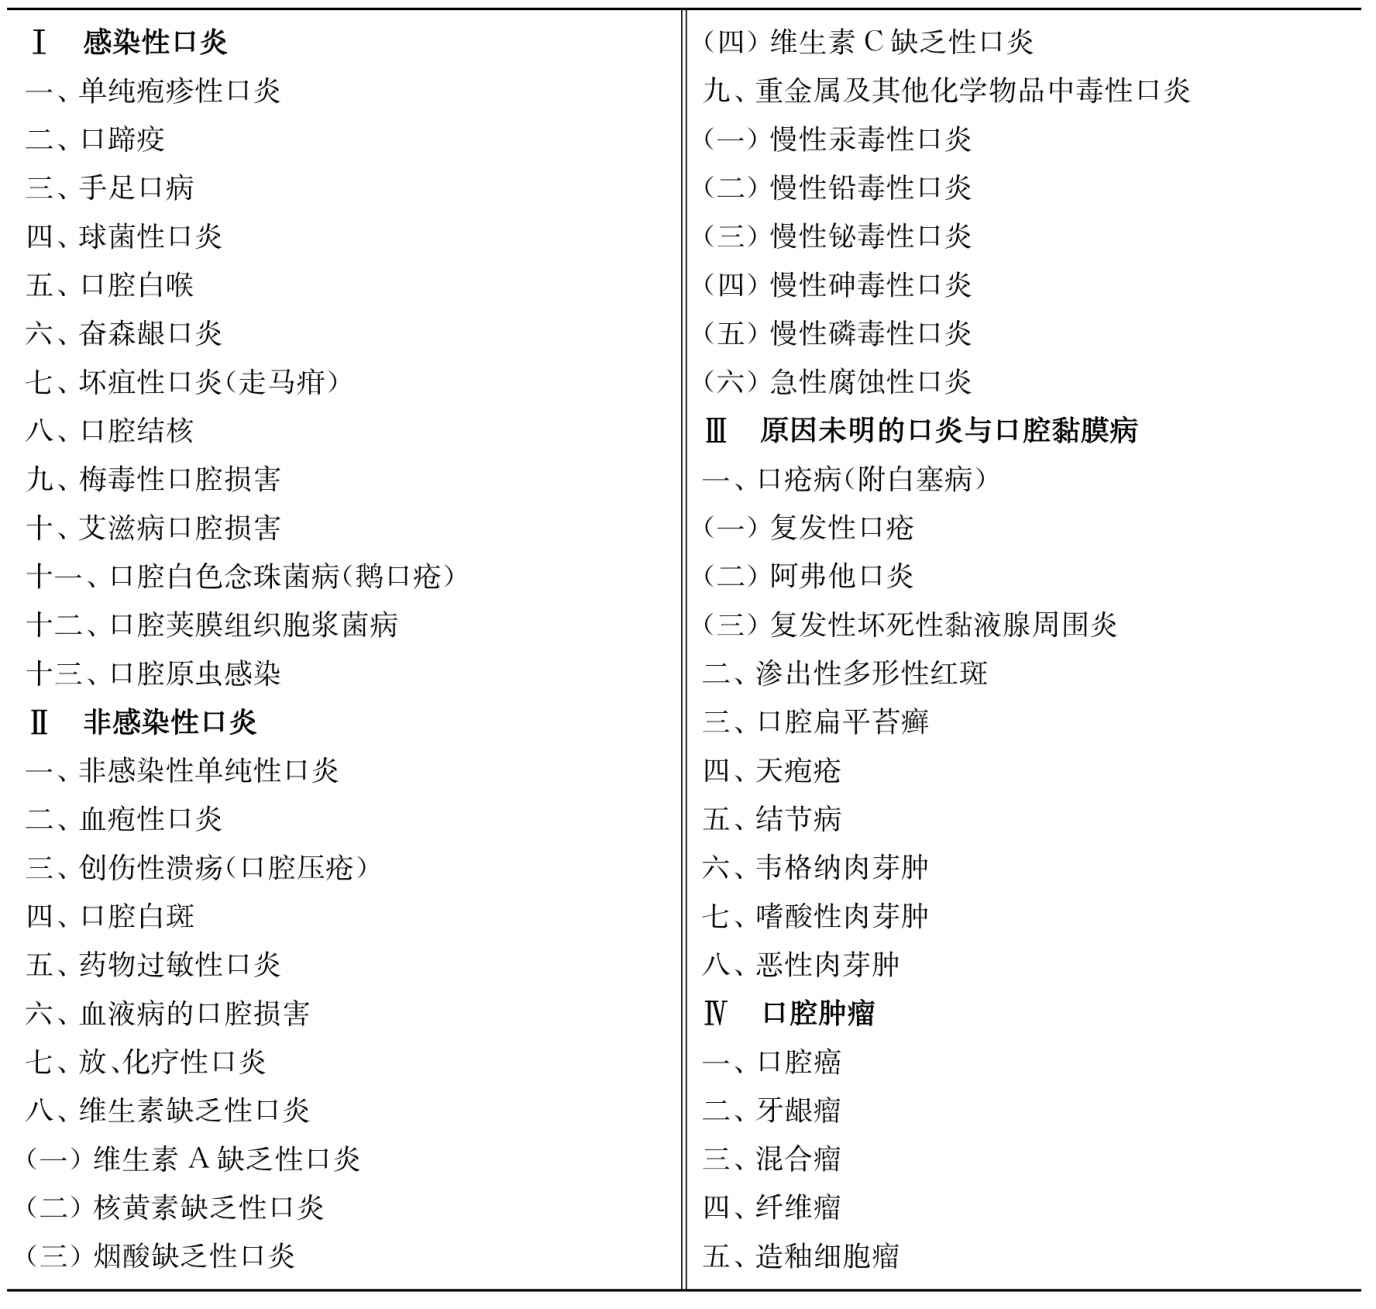
\includegraphics[width=5.91667in,height=5.625in]{./images/Image00113.jpg}
\end{table}

关于各种口炎方面,西安市几个医院统计的一组口炎发病率(表\ref{tab18-2}),可供参考。

\begin{longtable}{c}
 \caption{802例口炎的发病率}
 \label{tab18-2}
 \endfirsthead
 \caption[]{802例口炎的发病率}
 \endhead
 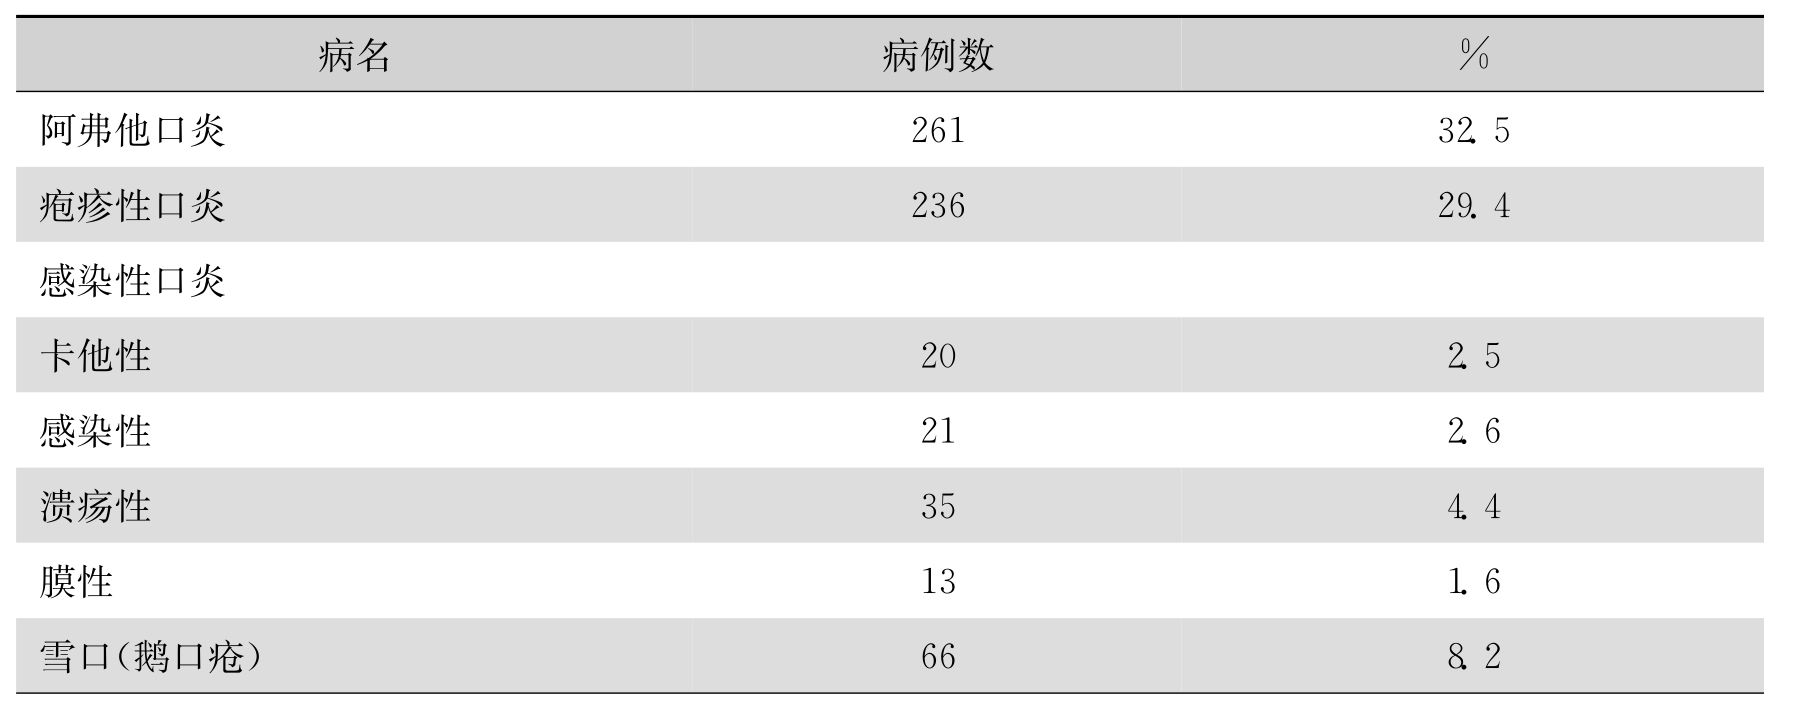
\includegraphics[width=\textwidth,height=\textheight,keepaspectratio]{./images/Image00114.jpg}\\
 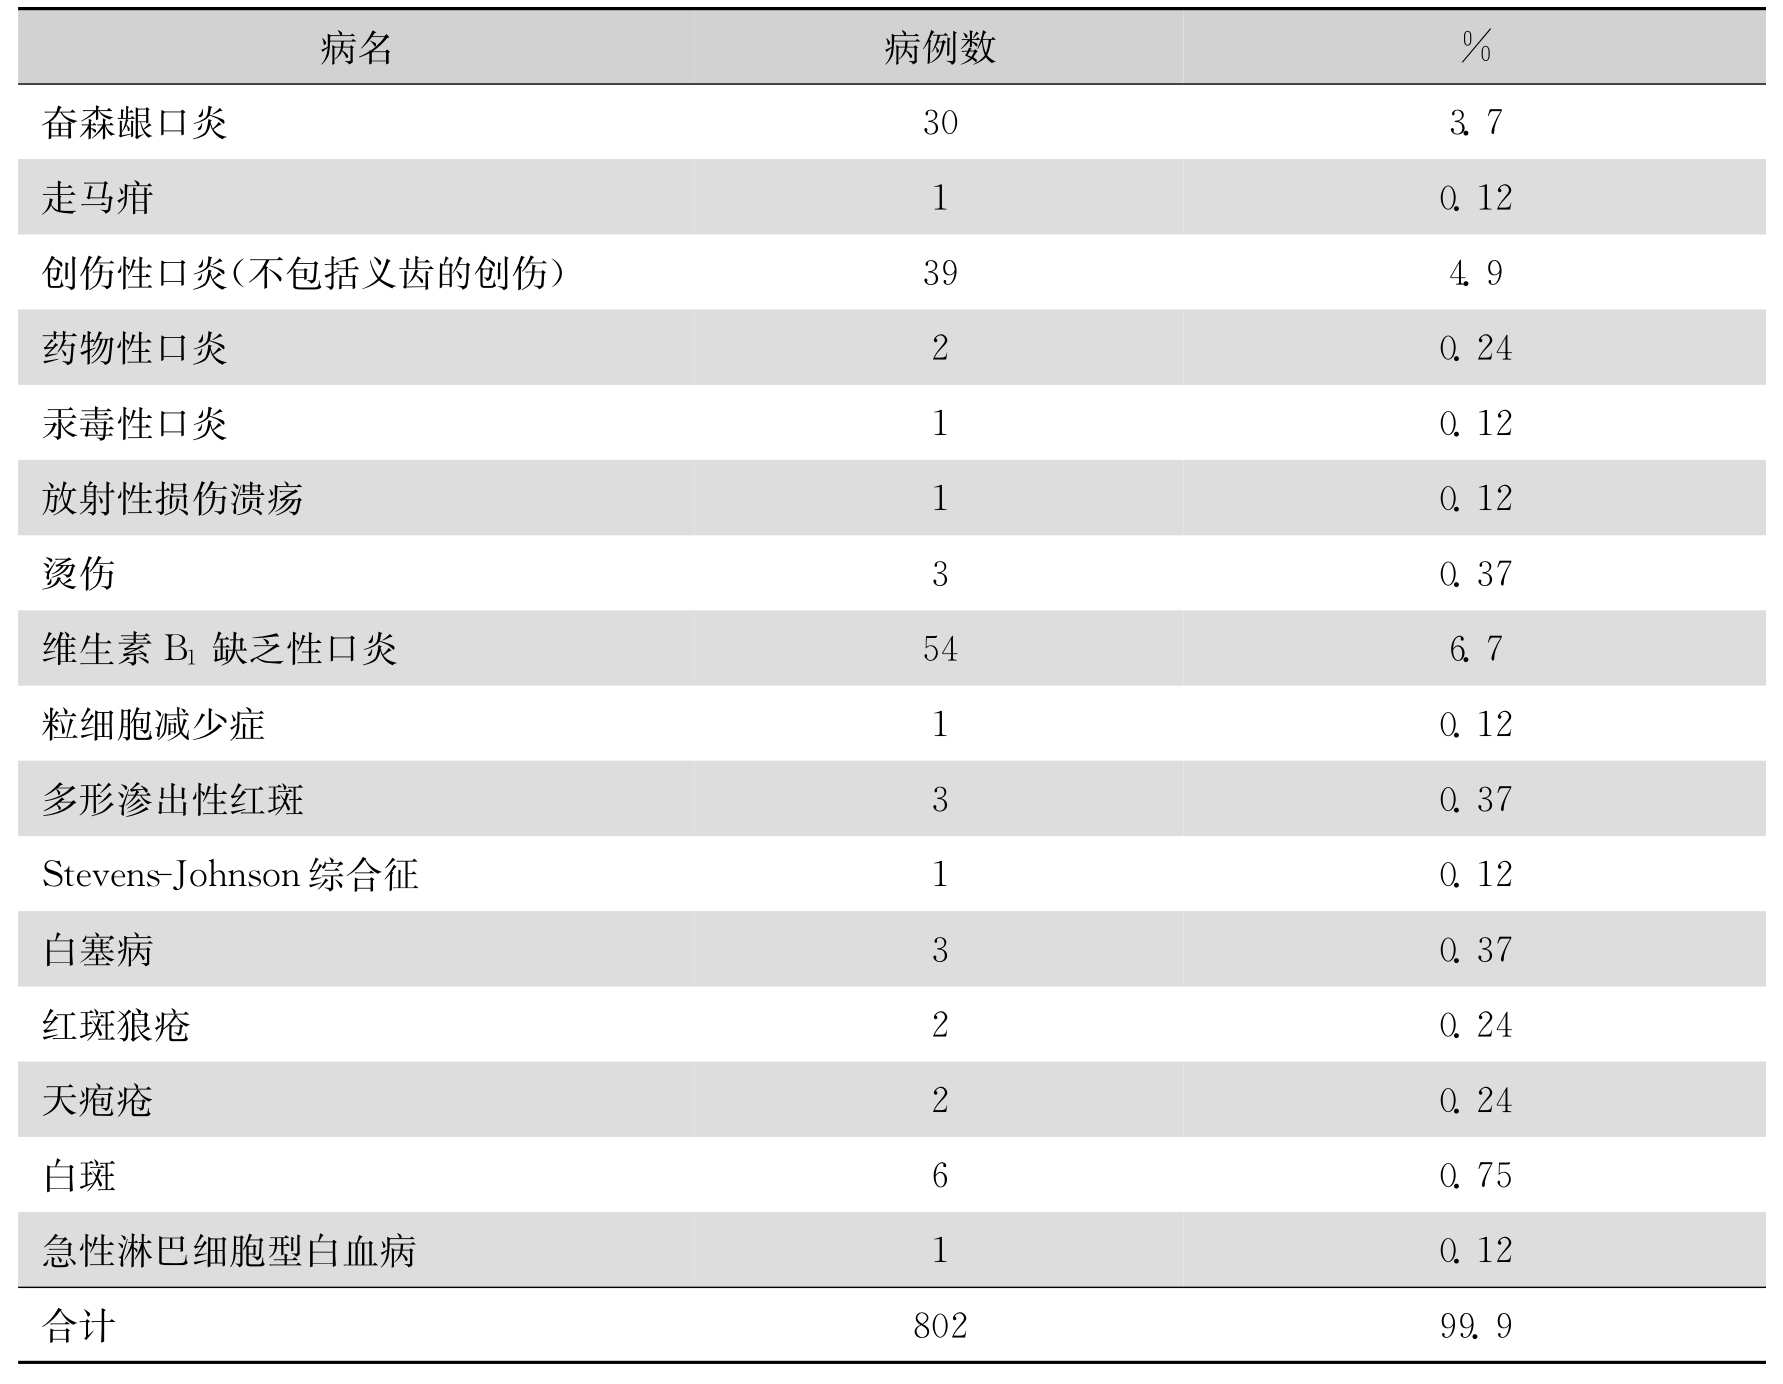
\includegraphics[width=\textwidth,height=\textheight,keepaspectratio]{./images/Image00115.jpg}
 \end{longtable}

\protect\hypertarget{text00149.html}{}{}

\section{56 感染性口炎}

\subsection{一、单纯疱疹性口炎}

据统计,在口腔炎症中,疱疹性口炎的发病率相当高,仅次于阿弗他口炎。儿童病例所占的比例更大,以6岁以下儿童多见,尤其是6个月至2岁更多。成人也有发作。发病季节以2~4月最多。

疱疹性口炎是由于单纯性疱疹病毒引起的口腔黏膜及口周皮肤的以疱疹为主的急性炎症。发热性疾病、感冒、月经、妊娠期、过度疲劳等均可为诱因。在疱疹出现前2~3天(潜伏期)常发现病儿烦躁、拒食、发热与颌下和颈部局部淋巴结肿大。口腔损害的最初表现为唇、舌、口腔黏膜与牙龈水肿以及弥漫性潮红,在24小时内渐次出现密集成群的灰白色或黄白色小水疱,多重叠,疱液大多澄清,好发于舌、颊黏膜、唇内侧与软硬腭等处。小水疱于2~24小时内破溃,形成帽针头或粟粒大小的溃疡。如几个小溃疡互相融合,则形成边缘不规则的、较大的溃疡。溃疡表面常被覆有黄白色分泌物,周围绕以狭窄的红晕。患者并有口腔烧灼痛、进食痛与口涎增多等症状。此病也有只发生在口唇的,称为疱疹性唇炎或口唇疱疹。

病程大多在1~2周之内,口腔黏膜损害渐次复常,溃疡愈合不遗留瘢痕。

此病首先须与三叉神经带状疱疹相区别。三叉神经带状疱疹也为病毒感染所致,患者多为成人,其分布限于一组神经所属的区域。可只有颜面皮肤发病,或单纯口腔黏膜发病,或皮肤与口腔黏膜均有损害,损害很少超越中线。疱疹较大、成簇,但不重叠,疱液变浑浊,甚至混有血液,短期内破裂形成溃疡面。溃疡存在时间较长,一般为2~3周,具有剧烈的疼痛,神经痛可延续1~2月之久,愈合后罕有复发。疱疹性口炎溃疡必须与阿弗他口炎相区别。阿弗他口炎的黏膜损害是几个分离的圆形或椭圆形小溃疡,直径为1~2mm至5~6mm不等,较深,中间略凹下,表面可有较厚的黄色或黄绿色被覆物,常发生于口腔黏膜转折处或舌边缘,比疱疹性溃疡更痛(表\ref{tab18-3})。

\begin{table}[htbp]
\centering
\caption{单纯疱疹性口炎与阿弗他口炎的鉴别}
\label{tab18-3}
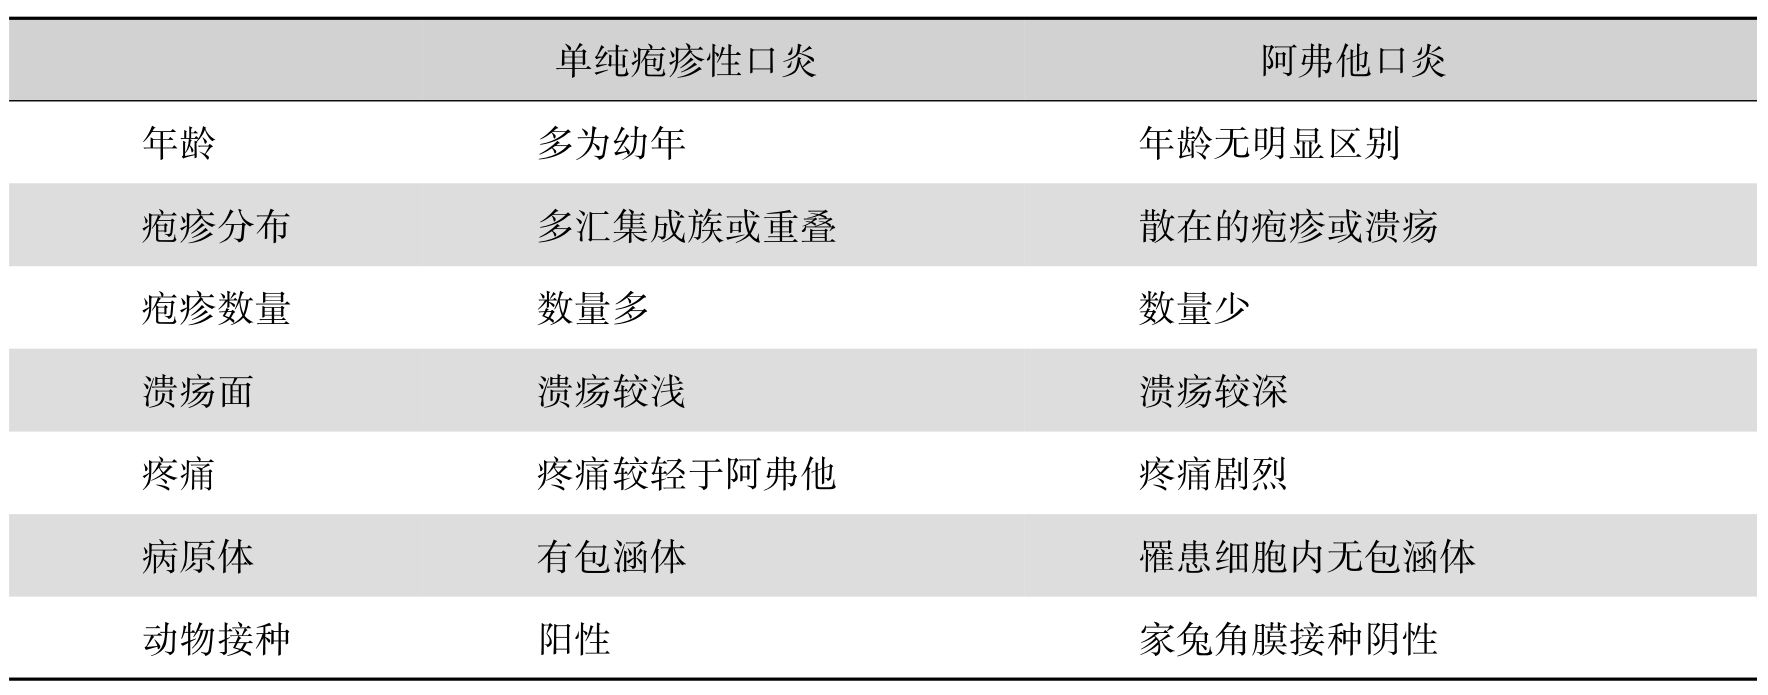
\includegraphics[width=5.88542in,height=2.30208in]{./images/Image00116.jpg}
\end{table}

\subsection{二、口蹄疫}

口蹄疫(aphthae
epizootic)是偶蹄类家畜------牛、羊、猪的一种急性口蹄疫病毒感染。人类也可受感染,但不敏感。偶尔畜牧区居民因进食受污染的食物、牛奶,或密切接触病畜而感染,国内曾有大批人被感染的病例报告,多见于成人牧民。潜伏期2~18天,继而出现发热、多涎,于口腔、咽喉、唇、舌等处黏膜及手掌、足底、指及趾间等处皮肤出现小水疱。数天后小水疱破裂,形成边缘不整的溃疡,被覆以灰黄色膜状物。溃疡痊愈后不留任何瘢痕。病程为自限性,一般为10天左右。诊断可根据流行病学史与临床表现。病毒分离及血清补体结合试验有特异性诊断意义。

\subsection{三、手足口病(hand-foot-and-mouth disease)}

多数是由柯萨奇和肠道病毒经飞沫、空气或消化道传播。日常接触被唾液、疱疹液及粪便污染的手、毛巾、玩具、食具、奶具以及床上用品、内衣等也可传播,接触被病毒污染的水源,可经口感染,并造成流行。好发于5岁以下婴幼儿及儿童,成人也可感染。全身症状轻微。口腔各部位均可出现疱疹及红斑。皮肤损害常见于手足,掌背均有,也可见于臀、腿、臂部,表现为红斑、丘疹及小疱。病程5~7天,有自限性。

\subsection{四、球菌性口炎}

葡萄球菌性口炎以儿童为多见,视诊可发现牙龈有暗白色苔膜,不易被拭去,但不致引起溃疡形成。口腔其他部位的黏膜有不同程度的充血。病儿可有轻度全身反应,并常有较明显的患部灼痛和流涎增多,局部淋巴结可有肿痛。涂拭物染色或培养证明有葡萄球菌(通常为金黄色葡萄球菌),即可确定诊断。

链球菌性口炎往往与链球菌性咽炎并发。在口腔黏膜急性充血的基础上,出现大小不等的黄白色苔膜,并伴有发热、不适感、纳差等全身症状。苔膜涂片或培养检查发现链球菌,即可确定诊断。

肺炎双球菌性口炎多发生于冬春两季,或气候骤变之际,老年人与儿童较易罹患。口腔黏膜初呈充血、水肿,继而出现银灰色斑状苔膜,伴有不同程度的全身反应,患部常有痛感。涂拭物涂片或培养发现肺炎双球菌而确定诊断。此病可与大叶性肺炎并发。

\subsection{五、口腔白喉}

原发性口腔白喉十分少见,且只见于幼儿。在冬、春二季发现幼儿有膜性口腔溃疡,伴全身症状者应加以注意,尤其是病程较长者,应做涂片或培养,检查白喉杆菌。

\subsection{六、奋森(Vincent)龈口炎}

奋森龈口炎是常见的口腔疾病,口腔护理不周的儿童或青少年发病率较高,致病菌为梭状杆菌与奋森螺旋体。发病以夏季最多。溃疡好发于牙龈与颊部黏膜,也可位于舌背、上腭等处,形态无定,大小多在1cm左右,大多浅表,被以污秽的、灰白色的苔。除去此苔膜时,出现溢血的溃疡面,但不久又再被覆以同样的苔膜。少数的溃疡较深,呈凿缘样,被覆以较厚不易剥脱的黄白色苔膜,周围明显充血。病灶有明显的触痛。

有特别强烈的坏死组织臭味,这种口臭是此病的特征。较重的病例并发颌下及颏下淋巴结不同程度的肿大与触痛,并有轻度或中等度发热、全身不适感、纳差等全身症状。

奋森龈口炎的经过可为急性或慢性,前者多见于小儿,后者多见于成年人。成年患者的全身症状一般较轻。

此病的确诊可根据特征性口臭、畏寒、发热、头痛、乏力等全身症状,龈缘、龈乳头红肿、溃疡、坏死出血,以及涂片中找到大量梭状杆菌与奋森螺旋体。此病鉴别诊断上须注意与急性白血病、粒细胞缺乏症、路德维咽峡炎等相区别。

路德维咽峡炎(Ludwig's
angina)是口底、颌下、咽部的一种弥漫性化脓性蜂窝织炎,病情发展异常迅猛,由其引起的败血症、中毒性休克等严重并发症较为常见。病因尚未明了,有人认为与螺旋菌或梭状杆菌有关。

\subsection{七、坏疽性口炎(走马疳)}

坏疽性口炎是一种进展迅速的坏疽病,好发生于极度全身衰弱的小儿,特别是重症急性热性传染病后。病因为螺旋体和梭状杆菌合并产气荚膜杆菌与化脓性细菌的感染。成年人罹患者极少,如有也仅见于重症全身性疾病的末期。病初在颊黏膜、齿龈或唇内侧发生紫红色斑,迅速转为紫黑色,触之稍硬,此即所谓原始焦痂。焦痂自行脱落后形成溃疡。坏死迅速向周围及深部发展,不久颊部皮肤也变为黑褐色,并溃破。坏死组织有特别强烈的恶臭。疼痛与发热较不显著。患者病情严重,如不及早救治,常于短期内因全身衰竭而死亡。

\subsection{八、口腔结核}

本病少见,可分溃疡型与增殖型(肉芽肿型),几乎都继发于开放性肺结核。肉芽肿型易被误诊为鳞癌,有时须反复活检方能确诊。抗结核治疗疗效甚佳。

患者多为体质较差的儿童、青少年和老人。溃疡型多表现为单个较深的溃疡,疼痛剧烈,最常发生于软腭、颊部及舌背等处。结核性溃疡的特点是边缘不整齐、凿缘样,基底不平滑、呈肉芽颗粒状,凸出部分呈红色,而凹陷部分呈微黄或浅紫色,溃疡周围组织缺少明显的炎性浸润,呈浅紫色。溃疡被覆物涂片或培养检查可发现结核菌。颈与颌下淋巴结常肿大。

诊断性抗结核治疗的较好疗效可证实口腔结核的诊断。病理组织活检也有助于诊断。

\subsection{九、梅毒性口腔损害}

由苍白梅毒螺旋体引起。一期梅毒特征性病损为硬下疳,唇部多见,其次见于舌、扁桃体,初发时粟粒大小,浸润性硬结,1~2周后,黄红至暗红的圆形或椭圆形溃疡,略隆起,无痛,溃疡基底平坦,触之软骨样硬结,相应区域淋巴结肿大、坚硬、无痛、不粘连。梅毒性口炎是二期梅毒病病征之一,一般在硬性下疳消失约2个月之后出现。口炎的发生可先于皮疹,也可晚于皮疹,或二者同时出现。整个口腔后部黏膜发生均匀的潮红充血,有时也可波及口腔前部黏膜。自觉症状不明显,主要表现为梅毒黏膜斑,为灰白色、光亮、微隆的斑块,直径0.5~1cm,圆形、椭圆形或环形损害,易发生糜烂、溃疡,但无疼痛。。三期梅毒形成梅毒性树胶肿,多位于舌、腭等处,可破坏腭骨而致口腔与鼻腔相贯通。梅毒性舌炎表现为舌乳头萎缩,表面光滑,经过度角化而发生梅毒性白斑。晚期先天梅毒可见桑葚状磨牙和新月状切牙。诊断主要根据上述的临床表现及梅毒血清学检查。

\subsection{十、艾滋病口腔损害}

口腔念珠菌病最为常见,常在早期就表现出来。特点:①发生于无任何诱因的成人;②常表现为红斑型或假膜型;③红斑型多发生于上腭和舌背,颊黏膜偶见;假膜型常累及附着龈、咽部、软腭、悬雍垂。毛状白斑对艾滋病有高度提示性。特点:①双侧舌缘的白色或灰色斑块;②常呈垂直皱褶,不能擦去;③需检测证实病损内疱疹病毒的存在。卡波西肉瘤是艾滋病最常见的口腔肿瘤,分为斑块期和结节期,女性患者少见。口腔疱疹若持续1个月以上,应做艾滋病的相关检查。艾滋病相关牙周病变有:牙周炎、牙龈线性红斑、坏死性牙龈炎,非霍奇金淋巴瘤在口腔好发于牙龈、咽部、腭,表现为高出黏膜面的软组织肿块,呈红色或紫色,有弹性,需经病理检查确诊。

\subsection{十一、口腔白色念珠菌病(鹅口疮)}

鹅口疮是口腔的白色念珠菌感染,呈急性或亚急性经过,罹患者常为衰弱的婴儿,也可发生于全身衰弱的成年慢性病患者。长期应用激素、广谱抗生素较易诱发此病。

鹅口疮初起时为隆起的针头大白点,出现于唇内侧、舌背面、颊、软硬腭等处的黏膜上,颇似残留的牛乳凝块,各点之间有正常黏膜间隔。发病不久,这些白点即互相融合成片,与基底粘连紧密,拭去易引起出血。患者多伴有低热、不适感、消化不良、腹泻等症状。此病如不迅速处理,任其继续发展,可蔓延至呼吸道、消化道,甚至引起真菌性败血症,其后果可甚严重。根据上述的临床表现,一般不难确定此病的临床诊断,可作口腔涂拭物涂片及培养检查以鉴定之。

\subsection{十二、口腔荚膜组织胞浆菌病}

本病临床表现为口腔黏膜与舌的溃疡,边缘不规则,有局部疼痛,并有进行性消瘦、贫血与白细胞减少。晚期多有不规则的发热。临床表现与口腔癌及结核性溃疡相似。国内有个别病例报告,此例经病理活检而确诊。本病以持续高热、肝脾大合并口腔损害的全身性感染也有报告。

\subsection{十三、口腔原虫感染}

齿龈阿米巴及口腔毛滴虫感染近年受到注意。原虫可从病灶或牙龈沟垢物涂片镜检发现。对顽固性口腔炎症,如抗生素治疗疗效不显著,而加用甲硝唑治疗有显著的疗效,亦符合本病的诊断。口腔护理不周、营养不良可成为口腔原虫感染的条件。

\protect\hypertarget{text00150.html}{}{}

\section{57 非感染性口炎}

\subsection{一、非感染性单纯性口炎}

非感染性单纯性口炎比较常见,不论任何原因的局部物理性、化学性、药物性、食物性或烟酒刺激,以及某些全身性疾病、妊娠期、月经期、便秘等,都可为发病因素。

患者常主诉口内发热感、进食乏味、口苦、有轻度口臭。望诊可见口腔黏膜潮红、水肿,失去正常光泽;有些病例可见到微白色苔膜,易被拭去,这是黏膜上皮表层坏死剥脱。病程中无溃疡形成。

\subsection{二、血疱性口炎}

机械性或热性刺激可能是此病的主要发病条件。血疱性口炎特别是在软腭部位突然发生圆形或椭圆形紫红色大血疱,继之自行破裂;破裂后形成类似假膜覆盖的创面,1~2天后假膜坏死脱落,形成圆形或椭圆形界限分明的大创面。创面略高于正常黏膜,底部有多数红点及毛细血管扩张,周围的黏膜有充血带。创面常因感染而有黄白色分泌物。患者常有局部疼痛与吞咽痛。如继发感染则有发热、头痛、全身不适感、颌下淋巴结肿痛等表现,约经10~21天而痊愈。

\subsection{三、创伤性口腔溃疡(压疮性口腔溃疡)}

创伤性溃疡是由于长期的机械性刺激或压迫所致的口腔软组织损害,通常由于托牙、卡环、破冠、残根、尖锐牙尖或牙缘的损伤所引起。由于外界的暴力作用、尖锐器械损伤所致的口腔溃疡也属于此范畴。溃疡发生于直接受损的部位,多见于舌的侧缘,也可发生于唇、颊及他处的黏膜,有自发性局部疼痛。溃疡表面覆盖以灰白色或浅黄色分泌物。如继发感染,则引起局部淋巴结肿痛。去除刺激因素后,病变通常在1~2周内痊愈。中年以上患者如不及时去除病因,慢性创伤性溃疡可为癌前病变。

如在慢性口腔溃疡基础之上出现硬结,或慢性溃疡去除病因一个月之后仍未愈合,须考虑癌变的可能,应即作病理活检以明确诊断。

\subsection{四、口腔白斑}

口腔白斑是因黏膜表层增生与过度角化,上皮的透明度减低,在罹患部位形成的白色斑片。触诊表面有粗涩感,失去正常的柔软和弹性。白斑的一般病理变化是上皮过度正角化或过度不全角化,有时为两种同时出现的混合角化。白斑的上皮增生分为上皮单纯性增生和上皮异常增生。国外报道患病率为3\%~5\%,国内报告偏高可能与诊断差异有关。病损范围可以小而局限,也可以是大面积而广泛分布。病损表面可为粗糙不平的皱纸状,或表面有颗粒样增生,或呈疣状隆起,或发生糜烂。一般无明显自觉症状。有些人有不适感,舔时发涩。多发生于40~50岁,罹患部位最多为颊黏膜,次为唇、舌黏膜。吸烟过多、饮烈酒、辛辣刺激品、维生素A、叶酸缺乏、口腔内持续的机械刺激、白色念珠菌感染、口腔慢性炎症、机体的内在因素等,均为白斑的发病诱因。白斑常被认为癌前病变,故发现患者有口腔白斑,应警惕发展为癌的可能性。如白斑基底变硬,出现皲裂、溃疡、出血,都可能是癌变的征象。

\subsection{五、药物过敏性口炎}

口炎可为全身性药物过敏性反应的局部表现(如Stevens-Johnson综合征),但有时也可仅表现为口炎(固定性药物过敏性口炎),而无全身性皮肤损害。临床上最常引起过敏性反应的药物是磺胺类、青霉素、巴比妥酸盐类与解热镇痛剂。甲氨蝶呤、6-MP、放线菌素D、博来霉素、硫酸长春新碱等抗癌药物,也可引起药物过敏性口炎。口腔黏膜损害可表现为充血、丘疹、水疱、结痂、溃疡与出血。常伴有不同程度的发热及局部疼痛、全身不适感、头痛、食欲减退、消化不良等症状。发病可急可缓,即发型在接受药物后几分钟至几小时发病,迟发型于接受药物后1天至2周左右发病。立即停药,口腔损害一般很快痊愈,再次用药时口炎又再发。鉴别困难者为无全身皮肤损害的药物过敏性口炎与局限于口腔的带状疱疹;后者沿口腔感觉神经分支而分布,很少越过中线,疱疹成小集落,有剧烈的疼痛,发病前无给药史。

\subsection{六、血液病的口腔损害}

血液病患者除因全身性与血液系统症状而就诊内科之外,尚有不少病例以口腔出血、牙龈肿胀、智齿冠周炎、口腔溃疡与疼痛而就诊于口腔科。牙龈肿胀,甚至表现为全口性牙龈肿胀,是急性白血病的重要口腔病征。龈缘渗血与黏膜出血常见于各类型血小板减少性紫癜。黏膜出血性大疱多见于急性型血小板减少性紫癜。各类型贫血均有不同程度的唇与口腔黏膜苍白。血友病患者常有拔牙后或乳牙脱落后不易止血的历史。坏死性口炎常见于急性白血病与粒细胞缺乏症,须与奋森龈口炎相鉴别。

\subsection{七、放、化疗性口炎}

放化疗后渐出现口腔干燥,唾液分泌减少,黏膜充血水肿,口腔局部可出现溃疡、坏死,牙齿松动,牙周炎发作,可有明显疼痛。故临床在头面部放疗和全身化疗前,应检查口腔,对可能造成的感染病灶,如牙周炎、牙龈炎、冠周炎、根尖周炎和坏死的牙髓预先处理,以防止局灶感染,甚至远隔器官的感染。

\subsection{八、维生素缺乏性口炎}

\subsubsection{(一)维生素A缺乏性口炎}

维生素A是脂溶性维生素,对皮肤、黏膜和某些腺体组织具有保护性和维持其功能的作用。维生素A缺乏时主要引起上皮组织的损害,特别是眼、口腔及皮肤。维生素A缺乏的口腔损害有牙龈过度增生、龈炎、牙周炎等,并可影响牙体组织发育,出现恒牙萌出迟缓、牙釉质发育不良、牙列不齐,而以下颌牙更为明显。

\subsubsection{(二)核黄素缺乏性口炎}

核黄素(维生素B\textsubscript{2}
)缺乏的临床表现主要局限于口腔与外生殖器,其中以口腔损害较早出现而明显,常有以下的病征:

\paragraph{1.对称性口角炎}

在两侧口角的皮肤和黏膜上出现乳白色糜烂,其后见有横纹裂缝,在过度张口或继发感染时出现疼痛。

\paragraph{2.唇炎}

一般表现为微肿、脱屑与色素沉着。偶有潮红、糜烂、裂隙、破皮、化脓或结痂。裂隙均为纵裂,有痛感。各种损害主要发生于下唇唇红部分。

\paragraph{3.舌炎}

早期舌尖的蕈状乳头及舌后的轮廓乳头肥厚,蕈状乳头表现为散在的针头大红点,舌肿大呈紫红色、干燥、有烧灼感或刺痛。后期丝状与蕈状乳头萎缩,舌面变为光滑,并出现散在性裂纹,舌色紫红(绛舌),舌痛常为突出的主诉。

\paragraph{4.口腔黏膜溃疡}

核黄素缺乏可引起阴囊红斑、丘疹、结痂、脱屑等损害,较重病例发生湿疹样阴囊炎,形态上与一般慢性阴囊湿疹相似,皮肤呈弥漫性浸润和变厚,间有渗液、裂隙与结痂,是较常见而有诊断价值的病征。

\subsubsection{(三)烟酸缺乏性口炎}

烟酸缺乏性口炎是糙皮病的部分表现,主要病变是不同程度的舌炎。病初时舌尖肿胀、潮红,继而蔓延及整个舌部,呈特别的朱红色,并出现舌痛。舌乳头消失。舌面可有小糜烂形成。病变进展时出现多数性小溃疡,其上覆以灰白色假膜,进食时感到剧痛,称为阿弗他口炎样烟酸缺乏性口炎。其与阿弗他口炎的鉴别要点为:小溃疡通常发生于舌背,无发疱期,病程长,无自限性,烟酸治疗有特效(表\ref{tab18-4})。其他系统症状为水样腹泻、胃酸减少或缺乏、全身裸露部分的对称性皮炎以及神经精神症状等。不少烟酸缺乏性口炎常继发奋森螺旋体与梭状杆菌感染,这是由于牙周组织抵抗力减弱所致。

\subsubsection{(四)维生素C缺乏性口炎}

维生素C缺乏时引起坏血病,牙龈损害表现为出血性龈炎,是最突出而早期出现的症状。病初时全部牙龈潮红、水肿,按之有如海绵,轻度接触即出血,或有自发性出血。继之常有溃疡出现,往往伴有疼痛与血腥样口臭。舌、腭弓、颊黏膜、舌边缘等处也可出现紫癜与血肿。女性患坏血病时,常有月经过多。长期缺乏维生素C是致病的原因。在此病的基础上,易继发奋森龈口炎。

\begin{table}[htbp]
\centering
\caption{阿弗他口炎样烟酸缺乏性口炎与阿弗他口炎的鉴别}
\label{tab18-4}
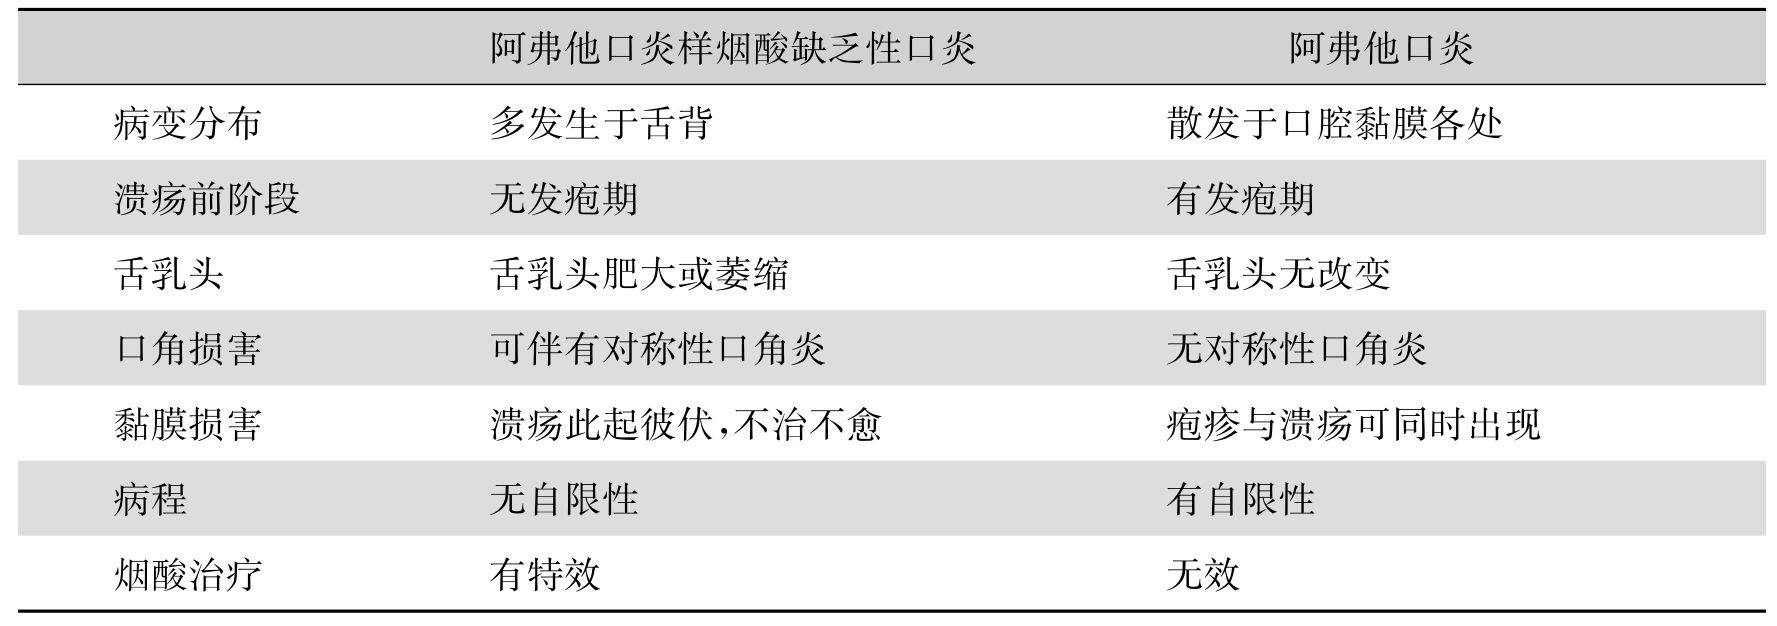
\includegraphics[width=5.91667in,height=2.07292in]{./images/Image00117.jpg}
\end{table}

此病在鉴别诊断上须注意与急性白血病及各类型紫癜相区别(参见第115节)。

\subsection{九、重金属及其他化学物品中毒性口炎}

重金属及其他化学物品中毒是某些工矿企业的职业病。汞、铅、铋等重金属以及砷、磷等进入人体之后,视摄入量的多少与摄入的快慢,可引起不同程度的中毒。临床上较多见的是长期小剂量摄入所致的慢性中毒,最重要的诊断根据是患者的职业史与接触史。除职业性中毒外,近年用含汞、铅的中草药偏方治疗银屑病、风湿病等症,医源性接触以及因使用含汞的美白去斑类化妆品经皮肤吸收的生活性汞、铅中毒时有报道,因其临床表现无特异,在综合性医院就诊患者不能提供明确的汞、铅等接触史,易被误诊、漏诊、误治,故需进一步提高对重金属中毒的认识。

\subsubsection{(一)慢性汞毒性口炎}

口炎是慢性汞中毒的早期症状,常先于其他症状而出现,主要表现为牙龈肿痛、流涎增多、口有金属味、牙龈易出血、齿槽脓漏。牙龈常有棕黑色的汞线,这是由于唾液中所含的汞,变为硫化汞沉着于此处所致。患者常有乏力、头昏、头痛、感觉异常、睡眠障碍、入睡困难、多梦、易醒、记忆力减退等神经衰弱症状。少数患者有嗜睡;部分患者则有性情急躁、易怒。上述临床表现可被误诊为神经衰弱。

患者有汞摄入史与上述表现,24小时尿汞排量≥0.25μmol/L(0.05mg/L)(双硫腙法),可诊断为慢性汞中毒。

\subsubsection{(二)慢性铅毒性口炎}

慢性铅中毒时,牙龈可出现铅线。铅线出现于牙龈唇颊舌侧的边缘上,距游离龈约1mm,呈宽约1mm的灰蓝色线条。牙龈常发炎,可有溃疡形成。患者自觉口有金属甜味,流涎增多。易并发奋森龈口炎。早期常有乏力、头晕、头痛、记忆力减退、睡眠不佳等神经衰弱症状。重症病例可出现腹绞痛、腹胀痛、肠梗阻与瘫痪,患者均可出现不同程度的贫血。

患者有铅摄入史与上述病征,24小时尿铅排量≥0.39μmol/L可诊断为慢性铅中毒。每百万个红细胞中点彩红细胞超过300个,也有诊断价值。常有尿卟啉阳性。

\subsubsection{(三)慢性铋毒性口炎}

慢性铋中毒的口腔早期病征,也为龈缘黑色金属沉着线------牙龈铋线。自觉症状不如慢性汞、铅中毒的显著,因铋盐对口腔黏膜的刺激性,远不及汞、铅的强烈。

\subsubsection{(四)慢性砷毒性口炎}

慢性砷中毒的口腔损害主要累及牙周部分。牙龈肿胀、充血、易出血,有时出现类似铅线的色素沉着。其他部分的口腔黏膜也充血、肿胀、糜烂或溃疡形成。患者感觉口干,有葱样臭味。其他病征为各种各样的皮疹、多发性神经炎、慢性消化道炎症与中毒性肝炎等。

\subsubsection{(五)慢性磷毒性口炎}

慢性磷毒性口炎主要表现为牙龈充血、肿胀、易出血。牙齿有针刺样、蚁走样或难以形容的疼痛。有蒜样口臭。可引起颌骨发炎、坏死、化脓、瘘管形成,出现所谓“磷毒性颌坏疽”。

\subsubsection{(六)急性腐蚀性口炎}

误服强酸或强碱等腐蚀剂可引起口腔黏膜灼伤、坏死与剧烈疼痛。酸类更可腐蚀牙齿。剂量较大的腐蚀剂可引起消化道黏膜灼伤与坏死,严重者发生休克与穿孔。如能治愈,常遗留消化道(主要是上消化道)瘢痕性狭窄。

\protect\hypertarget{text00151.html}{}{}

\section{58 原因未明的口炎与口腔黏膜病}

\subsection{一、口疮病}

口疮病出现于口腔黏膜上,是常见口腔病之一。一般初发年龄在10岁左右,21~30岁是复发最频繁的阶段。此病在临床上有下列三种表现:

\subsubsection{(一)复发性口疮}

复发性口疮或称阿弗他溃疡,其最初表现是在口腔黏膜,特别是唇、舌与颊黏膜上出现小水疱,直径一般在2mm左右,单个或二、三个,约经6~12小时后而自行破裂,形成小溃疡。溃疡呈圆形或椭圆形,直径数毫米,表面凹陷,有灰白色膜状物,边缘稍隆起,具有强烈的疼痛,每当食物的刺激而加重,但患者全身症状一般不明显。病程为自限性,溃疡通常经数天而逐渐愈合,一般为7~10天,但甚易复发,往往延续多年。

\subsubsection{(二)阿弗他口炎}

阿弗他口炎多发生于10岁左右的儿童,但成年人也可罹患。此病有复发的倾向,全身症状随年龄增长而减轻。

疱疹出现之前,患者常有全身不适感、乏力、头痛、纳差、畏寒与不同程度的发热(可达40℃)等全身症状,继而在唇颊内侧、舌面、上腭等处出现散在性多数性小水疱,一般自八、九个至十余个不等。水疱不久穿破而形成小溃疡,全身症状逐渐缓解,但局部疼痛反而加剧,并伴流涎增多。局部淋巴结可发生肿痛。溃疡约经10~14天而愈合,不留瘢痕。

阿弗他口炎须与单纯疱疹性口炎以及烟酸缺乏性口炎相区别。

\subsubsection{(三)复发性坏死性黏液腺周围炎}

此病临床上少见,多发生于青年,国内仅有少数病例报告。其临床特点是病初时在黏膜下层出现单个的小结节,逐渐扩大与坏死而形成小溃疡。溃疡可增大至1~2cm,偶尔达4cm,一般位于口角后端、舌尖、舌缘和颊黏膜等处,多次复发后溃疡逐渐向后移,达软腭、咽壁及腭垂等处。溃疡的特点是大而深、边缘不整齐而较硬,中部凹陷,被以黄色假膜,溃疡周围无红晕,疼痛剧烈,愈合较慢,病期达2~3个月甚至更长,愈合后往往遗留白色线状瘢痕,但常无明显的淋巴结反应。此病须注意与口腔癌性溃疡相区别(表\ref{tab18-5}),如未能除外后者,应尽早做病理组织活检。

\begin{table}[htbp]
\centering
\caption{复发性坏死性黏液腺周围炎与口腔癌性溃疡的鉴别}
\label{tab18-5}
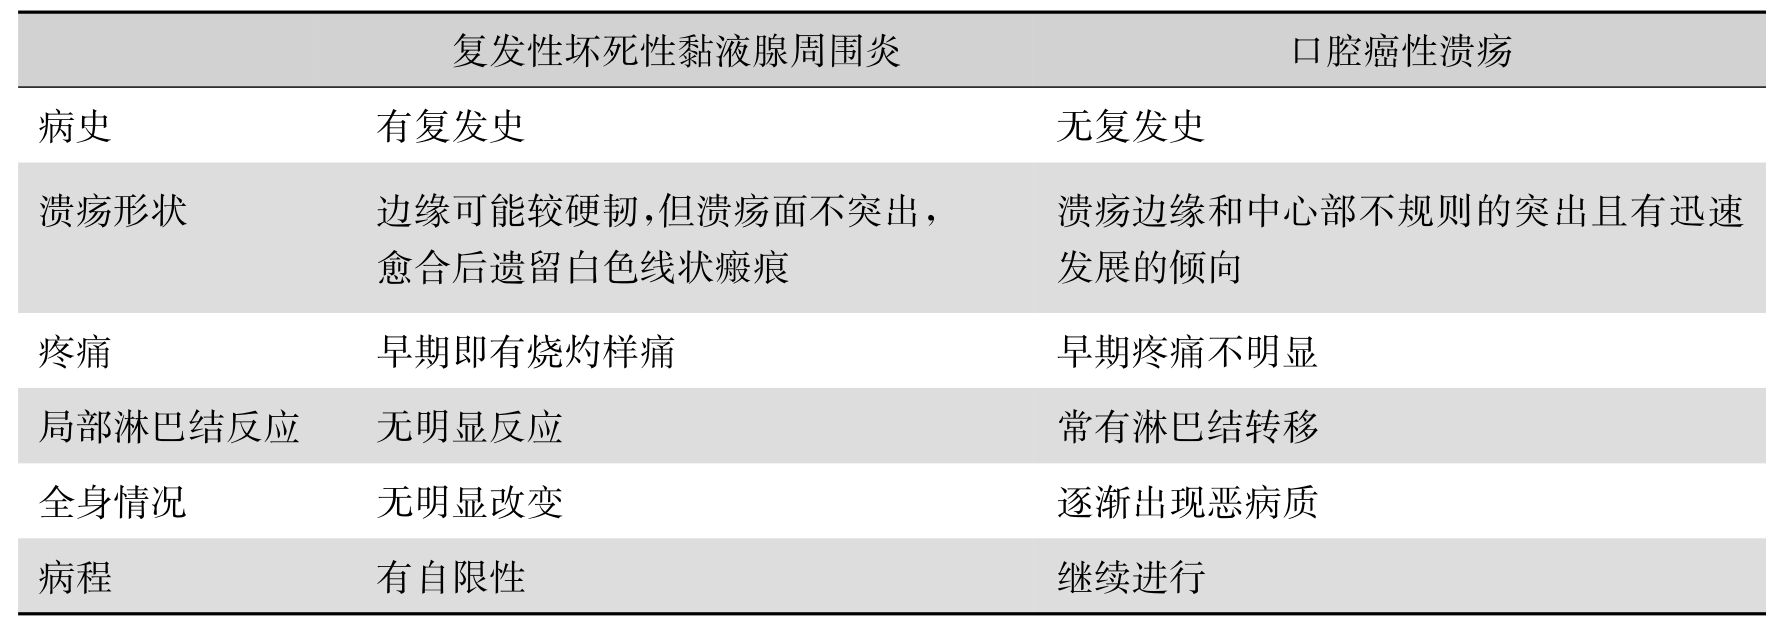
\includegraphics[width=5.91667in,height=2.07292in]{./images/Image00118.jpg}
\end{table}

\subsubsection{附:白塞病(Behcet disease)}

白塞病并非少见,2/3有口腔损害。本病以慢性经过,反复发作为临床特征,临床表现多样化,但主要表现为阿弗他口炎伴有外生殖器疱疹与溃疡、眼部病变(虹膜睫状体炎、角膜炎、葡萄膜炎、视网膜血管炎、前房积脓等)、皮肤病变等。不少病例先由眼科、口腔科或皮肤科医生发现。发热、全身不适和关节痛是常见的症状。

口腔损害主要是散发性多数性小溃疡(口疮),多呈圆形,伴有明显的自发痛,常发生于口唇、舌尖、舌侧缘、齿龈等处,咽部较少。口腔溃疡的特点是发生早,发病率高,常反复发作,无长期缓解。

外生殖器损害与口腔损害基本相同,呈大小不一的小溃疡,伴有明显的炎症反应与疼痛,发病部位男性多在阴囊,其次为阴茎、龟头、冠状沟等处,女性多发生于大、小阴唇,多为数处并发。

眼部病变半数有之,主要表现为复发性虹膜睫状体炎、前房积脓、虹膜炎、视网膜炎、葡萄膜炎、角膜炎或溃疡、结膜炎等病变。

2/3以上病例有皮肤损害,以结节性红斑样皮疹为多见,此外为毛囊炎样损害、痤疮样损害(患者用糖皮质激素)等。患者虽在严格灭菌操作下接受皮肤针刺(如皮下、肌内或静脉注射),屡次在针刺部位发生小脓疱,此症状对提示诊断有重要意义。

在内科表现方面,本病可出现血栓性静脉炎与血栓性动脉内膜炎,并由此引起中枢神经系统损害(脑膜脑炎征、瘫痪、精神失常等)、心血管病变(动脉瘤、三尖瓣病变)以及肢体的静脉血栓形成与肺栓塞等,还可有关节痛、发热、非特异性消化道溃疡等表现,有食管、胃、小肠、大肠溃疡性病变表现者,还需特别注意与克罗恩病,甚至淋巴瘤鉴别。

本病的表现复杂,口腔溃疡、关节炎、血管炎可在多种风湿疾病出现。有时各局部病征发生的间隔与时间均无一定的规律性,因此对部分病例的诊断,仍有赖于临床细致观察和分析,而不应为诊断标准所束缚。

据第八届国际白塞病学术会议制定的诊断标准为:患者有复发性口疮溃疡每年至少发作三次,并具有下列各项中至少两项相继发生或同时出现:①外生殖器溃疡;②眼病;③皮肤病变;④针刺试验阳性。

\subsection{二、渗出性多形红斑}

本病病因尚未完全明了,目前认为是变态反应性疾病,具自限性,可复发,多见于春、秋两季,与感染、药物、食物过敏等有关。

临床特点是以不同程度的全身前驱症状而起病,于四肢皮肤(特别是手背、关节曲面)、外生殖器、肛门周围、眼、口腔黏膜等处,出现红斑、丘疹、水疱、结痂与溃疡形成。红斑的周围可有红色圈,如环状。红斑中心常有小疱疹,不久结成浅褐色痂。若多数的大小环相套,各色相间,形如彩虹时,则称为虹样红斑。发疹大多累及口腔黏膜,且口腔损害往往较其他部分的损害严重,或口腔单独发病。颊两侧、唇、舌面、舌底、口底、腭等处均为好发部位。唇部由于皲裂与经常活动,有时出血较重,出现黑色血痂,是本病特征之一。

本病临床上可分为轻型(Hebra型)与重型[斯-约(Stevens-Johnson)综合征]二型。前者发疹少,病程短,症状较轻。后者发病急,常有恶寒或寒战、高热,病情重,病变也较广泛,可遍及全身,甚至危及生命。国内曾有个别病例报告,因苯巴比妥或长效磺胺过敏引起而死亡者。

\subsection{三、口腔扁平苔癣}

扁平苔癣是一种非感染性慢性炎症性皮肤与黏膜病,病因尚未明了。口腔黏膜病中除复发性口腔溃疡外,以扁平苔藓最为常见。国内报告发病女多于男,罹患最多为20~50岁。病理表现为上皮过度角化或不全角化,上皮角质层增厚或变薄,粒层明显,基底细胞液化变性,基膜下方可见大量淋巴细胞浸润带。上皮固有层可见均匀嗜酸染色的小体。此病很少发生癌变。约50\%皮肤与黏膜同时受累,但不少单独发生于口腔黏膜,好发于颊面、舌面、唇内、牙龈等处,且多为对称性累及颊部黏膜。

颊扁平苔癣可为双侧性或单侧性,位于合线或颊沟。病区有珠光色或灰白色点状小丘疹,连续成线纹状;线纹互相交织成网状、环状、花边状等不同形态。在灰白色小丘疹周围的黏膜无明显的炎症。可无明显自觉症状。有时病灶的黏膜出现糜烂,可觉疼痛。

舌扁平苔癣主要位于舌前2/3的舌背和边缘,呈圆形或椭圆形、边缘整齐的斑状或花边状病区。斑状病区的中部为浅灰白色薄膜,但仍显示正常的乳头,故与白斑有所区别。患者除有痒感之外,无其他自觉症状。

如口腔扁平苔癣与皮肤病变同时出现,诊断比较容易,但如单独出现的不典型的口腔病变,则诊断比较困难。皮肤损害多见于前臂、手腕、下肢、颈部,也可发生于腰、腹、躯干及生殖器。表现为散在或成簇针头大小的红色多角形扁平丘疹,也可为绿豆或黄豆大小丘疹,开始为粉红、红色,逐渐变成紫红或紫蓝色,丘疹表面扁平略凹陷,边界清楚,表面有蜡样光泽,上覆鳞屑。

口腔扁平苔癣主要须与口腔白斑相区别。白斑不伴皮肤损害,两者的病理变化也不同。诊断根据是本病特有的小丘疹,以及由此形成的灰白色网状或花边状线纹,触诊病变黏膜表面仍柔软有弹性,无粗涩感,但有时须经病理活检方能鉴别。

\subsection{四、天疱疮}

天疱疮是少见而严重的皮肤病,病因未明,现多认为是自身免疫性疾病,临床分为寻常性天疱疮、增殖性天疱疮、落叶性天疱疮、红斑性天疱疮四个类型。各型损害情况虽然表现不同,但均有棘层松解这一病理特征。多发生于中年以上,40~60岁较常见。其特征是在皮肤、口腔黏膜、咽黏膜等处发生多数大小不等的水疱。口腔黏膜为好发与早发的部位,皮肤多见于头皮、胸背躯干、腹股沟等易受摩擦部位。水疱的直径自数毫米至十数毫米或更大,疱壁甚薄,数分钟至十数分钟即可自行破裂。破裂后出现圆形或椭圆形糜烂面或浅在性溃疡,并有显著疼痛。进食、咀嚼与吞咽等动作均受妨碍,严重影响患者的营养状况。对外观正常的皮肤或黏膜加压刺激或摩擦后,易形成疱或脱皮,轻压疱顶可使疱向四周扩展,这种现象称尼氏征(Nikolsky's
sign)。在病情发展阶段,患者常有畏寒、发热、食欲减退等全身症状。皮肤与口腔黏膜水疱此起彼伏,直至全身衰竭。

\subsection{五、结节病}

结节病是一种全身多系统及组织器官发生的非干酪样坏死性上皮样肉芽肿性疾病。其临床上主要表现为双侧肺门淋巴结肿大及肺部侵犯,也可侵犯皮肤、眼、浅表淋巴结、肝、脾、肾、骨髓、心脏和神经系统等器官,口腔以唇颊部常见,唇组织增厚肿胀,形成巨唇,触诊有硬结。血管紧张素转换酶(SACE)水平明显升高。诊断需排除其他非干酪样坏死性肉芽肿疾病。

\subsection{六、韦格纳肉芽肿}

是一种特征为坏死性肉芽肿性表现的疾病。临床表现开始于上呼吸道,可表现为鼻窦炎、鼻出血,经常有肾脏损害,可有发热、乏力、关节痛等。口腔黏膜出血坏死性肉芽肿性溃疡,好发于咽和软腭,可破坏骨组织。

\subsection{七、嗜酸性肉芽肿}

因刺激因素引起的反应性增殖性炎症性病变。多见于舌,也见于牙龈、腭、唇处的黏膜,表现为边缘不整的黏膜溃疡。病理活检为大量嗜酸性粒细胞浸润。

\subsection{八、恶性肉芽肿}

恶性肉芽肿又称致死性中线性肉芽肿(lethal midline
granuloma),好发于青壮年男性。病因未明,病变一般先侵犯鼻腔,以后侵及鼻咽及口咽部。

恶性肉芽肿的主要临床与病理特点是面部近中线的慢性进行性非特异性肉芽组织增生与坏死,累及鼻、咽、上腭、喉头等处,以致最后形成整个面部的损坏、大出血、内脏损害与全身衰竭。进行性病例常有不同程度的发热,多呈弛张型或不规则型。当患者尚无显著的内脏损害时,虽有鼻咽与口咽部严重病变及高热,但食欲、精神及全身情况仍较良好,与一般感染性疾病及晚期恶性肿瘤有所不同。

此病的主要诊断根据是:①侵犯面部近中线的慢性进行性溃疡;②局部症状(以及全身情况)与局部病变不成正比例,局部可能有广泛的破坏,而自觉症状较轻微,全身情况也较好;③局部(颌下与颈部)淋巴结一般无明显肿大;④病理活检所见为炎症性肉芽组织;⑤各种细菌血清学检查包括梅毒血清反应、结核杆菌检查等均为阴性。恶性肉芽肿的诊断主要依靠排除诊断法。如患者经反复活检均证明为炎症性肉芽组织与坏死组织,而临床表现与上述情况相符,细菌血清学检查也无特异性炎症的证据,可诊断为此病。

恶性肉芽肿可侵犯内脏,但此病与韦格纳(Wegener)肉芽肿不同。韦格纳肉芽肿的病理特点为坏死性肉芽肿中的小血管炎和小血管周围炎,且构成血管炎的浸润细胞主要为淋巴细胞,肉芽组织中还可见有朗格汉斯细胞,偶见上皮样细胞,且病变常累及肺、肾、皮肤、眼、关节等器官,这些情况在恶性肉芽肿罕见,并有助于二者鉴别。韦格纳肉芽肿死亡原因最常为肾功能衰竭,而恶性肉芽肿死亡主要由于营养不良、出血与败血症。用ANCA技术诊断韦格纳肉芽肿,特异性为86\%,敏感性为78\%,可与恶性肉芽肿相鉴别。参考第5.3节。

\protect\hypertarget{text00152.html}{}{}

\section{59 口腔肿瘤}

常见的口腔肿瘤有下列几种,其诊断主要依靠活体组织检查。

\subsection{一、口腔癌}

口腔癌的发病率颇高,大多数为鳞状上皮癌,41~70岁发病率最高,男女发病比率约为2∶1,罹患部位以龈癌占首位,舌癌次之,腭癌、颊癌又次之,唇癌较少见。癌组织富于毛细血管,因此易引起出血,有易于形成溃疡的倾向。典型的癌性溃疡质硬,边缘隆起、呈堤围状而不整齐,基底也凹凸不平。口腔癌的转移率平均为40\%,2/3发生颈淋巴结转移。

\subsection{二、牙龈瘤}

过去曾将一切发生于牙龈的肿瘤都称为牙龈瘤,但近来对牙龈瘤的定义,是指发生于牙槽突上的炎症性增生物。

牙龈瘤易发生于青壮年,但40岁以后的发病率也不低,男女比率约为1∶2,多发生于牙龈的唇颊侧,均属良性肿瘤。病理组织学上以肉芽肿型及纤维型牙龈瘤占多数;血管瘤型牙龈瘤较少见,病理改变为毛细血管增生与扩张。

\subsection{三、口腔混合瘤}

口腔混合瘤任何年龄均可罹患,但以31~50岁最多。此瘤最多发生于腭部。肿瘤生长缓慢、局限性,大小不一(可为拇指头大或鸡蛋大),表面光滑或有结节状突起,较硬,而发生黏液性变或囊性变时则较软。被覆的黏膜正常。如癌变则表面易发生溃疡,并侵犯邻近组织和器官,但淋巴与血行转移者很少。

\subsection{四、口腔纤维瘤}

纤维瘤是常见的口腔肿瘤之一,是一种良性瘤,可发生于牙槽黏膜,腭黏膜、唇、颊、舌黏膜,以及上、下颌骨。此瘤发展缓慢,质软或硬,有蒂或无蒂,表面大多平滑,有时也呈结节状。任何年龄均可罹患,而以21~30岁较多见。女性罹患略多于男性。诊断须根据肿瘤活体组织检查。

\subsection{五、造釉细胞瘤}

造釉细胞瘤是一种上皮肿瘤;通常为良性,多发生于青壮年人的下颌骨。此瘤发展缓慢,初期几无症状,经过多年,当肿瘤长大时,可压迫下齿槽神经而出现疼痛或麻木感。位于上颌者可侵入上颌窦内。发展较快者多为分化度低而具有恶性的类型,可转移至颌下淋巴结与颈淋巴结。

\protect\hypertarget{text00153.html}{}{}

\section{参考文献}

1.郑际烈.血液病之口腔表征22例报告.中华口腔科杂志,1965,11:297

2.陆道培,等.遗传性出血性毛细血管扩张症.中华医学杂志,1973,53:543

3.方荣柳,等.黑毛舌与内科有关的几个问题.中华口腔科杂志,1965,11:322

4.盛履谦,等.802例口炎初步分析报告.中华口腔科杂志,1959,7:1

5.于长水.手足口病流行及研究进展.中华传染病杂志,1989,7:35

6.王德恒.手足口病1026例临床分析.天津医药,1983,11:740

7.张永福,等.走马疳12例及其后遗症68例分析.中华口腔科杂志,1965,11:38

8.黄逸民.口腔结核性溃疡21例的分析.中华口腔科杂志,1965,11:375

9.刘玉峻,等.口腔黏膜结核38例临床分析.天津医药,1980,8(9):559

10.周平,等.口腔黏膜结核的临床分析.中华结核和呼吸杂志,1998,21(4):251

11.吴忠,等.路德维氏咽峡炎合并中毒性心肌炎八例.中华心血管病杂志,1997,25:153

12.董怡,等.原发性干燥综合征诊断标准的初步探讨.中华内科杂志,1996,35(2):114

13.李哲.西安市572人齿龈阿米巴及口腔滴虫感染.中华口腔医学杂志,1988,307

14.丁良驹,等.血泡性口炎(附17例分析).中华口腔科杂志,1965,11:77

15.戴策安,等.口腔白斑的病因分析、临床病理及其防治措施.中华口腔科杂志,1964,10:316

16.陆先韫.口腔白斑.中华口腔科杂志,1980,15(2):103

17.王正坤.天津市31961例口腔白斑调查.天津医药,1983,11:589

18.黄正吉.白塞氏病310例的研究报告.中华内科杂志,1982,21:331

19.陈寿坡,等.Behcet氏病的一些特殊临床表现------病例报告和文献综述.中华内科杂志,1980,19(1):15

20.董怡,施桂英.第八届国际白塞病学术会议简介.中华内科杂志,1999,38(2):135

21.马莉,等.以消化道损害为首发症状的贝赫切特综合征11例临床分析.中国综合临床,2003,19(11):1004

22.罗永立,等.组织胞浆菌六例.中华内科杂志,1998,37(3):303

23.贺凌飞,等.艾滋病患者的口腔损害及其在艾滋病诊断中的作用.华中科技大学学报(医学版),2002,31(3):346

24.彭式韫,等.口腔黏膜扁平苔癣.中华口腔科杂志,1965,11:7

25.李辉奉.口腔扁平苔癣.中华口腔科杂志,1980,15(2):88

26.石嘉玲,等.恶性肉芽肿在眼部、皮肤和全身的表现.中华医学杂志,1974,54:437

27.中国医学科学院肿瘤研究所.坏死性肉芽肿.中华医学杂志,1974,54:242

28.朱元珏.Wegener肉芽肿和中线坏死性肉芽肿.中华内科杂志,1984,23:407

29.陈文彬.致死性中线肉芽肿.中华内科杂志,1986,25:142

30.李龙芸,等.肺血管炎和肉芽肿病.中华内科杂志,1992,31:424

31.叶国钦.口腔幽门螺杆菌感染的处理策略---必须面对的一个重要问题.中华医学杂志,2012,92(10):659

32.李蓬,等.伴牙周炎的代谢综合征者动脉硬化早期指标的检测.北京大学学报(医学版),2011,43:34

33.和璐.牙周炎和代谢综合征.北京大学学报(医学版),2011,43:13

34.章锦才.慢性牙周炎影响糖尿病发生及发展的研究进展.中华口腔医学杂志,2013,48(3):138

35.孙涛.肝硬化出血相关预测因子分析.中华内科杂志,2012,51(6):424

36.李敏,等.炎症性肠病的口腔损害及其诊断.国际口腔医学杂志,2010,37(3):330

37.陈渊,等.长期不愈口腔溃疡的致病因素分析与诊断思路.现代口腔医学杂志,2013,27:44

38.刘晓玲,等.汞中毒92例临床分析.中华内科杂志,2011,50(8):687

39.郭涛,等.铅中毒七例临床分析.中华内科杂志,2009,48(9):767

\protect\hypertarget{text00154.html}{}{}

